\documentclass[
  % all of the below options are optional and can be left out
  % course name (default: 2IL50 Data Structures)
  course = {{IE579 Game Theory and Multi-Agent Reinforcement Learning}},
  % quartile (default: 3)
%   quartile = {{3}},
  % assignment number/name (default: 1)
  assignment = 1,
  % student name (default: Some One)
  name = {{Mohammad Mahdi Rahimi}},
  % student number, NOT S-number (default: 0123456)
  studentnumber = {{20208244}},
  % student email (default: s.one@student.tue.nl)
  email = {{mahi@kaist.ac.kr}},
  % first exercise number (default: 1)
  firstexercise = 1
]{aga-homework}

\usepackage{amssymb,latexsym,amsmath,amsthm}
\usepackage{amsfonts,rawfonts}
\usepackage{thmtools}
\usepackage{systeme}
\usepackage{mathtools}
\usepackage{pgfplots} 
\pgfplotsset{width=10cm,compat=1.9} 
 \usepgfplotslibrary{external}

\tikzexternalize 

\begin{document}

\exercise
\subexercise Formulation of Game

Players are P1 and P2\[ n = 2\].

Action for each Player define a Real number in \[A = \{ a | a \in [0,100] \}\]

Payoff Function for Players:
\[ U_{P1} = 
     \begin{cases}
       a_1 &\quad\text{if }a_1 + a_2 \le 100 \text{ or } a_1 < a_2\\
       100 - a_2 &\quad\text{else if } a_1 > a_2 \\
       50 &\quad\text{otherwise}\\ 
     \end{cases}
     U_{P2} = 
     \begin{cases}
       a_2 &\quad\text{if }a_1 + a_2 \le 100 \text{ or } a_2 < a_1\\
       100 - a_1 &\quad\text{else if } a_2 > a_1 \\
       50 &\quad\text{otherwise}\\ 
     \end{cases}
\]

\subexercise Proof (50, 50) is a Nash Equilibrium
\\

Assume we are currently in (50, 50) situation and this is not a Nash, so there is exist a player that can improve its own payoff by changing action.
As situation is symmetry regards to players, we assume P1 will change the action.
\\

If P1 increase the amount, it leads to situation where summation of amount pass 100 limit and P1 receive 50 again. 
\\

If P1 decrease the amount, it leads to situation where summation of amount not passed 100 limit and P1 receive less than 50.
\\

In either way nor P1 or P2 can increase the payoff by changing actions, so it's Nash equilibrium.
\newpage
\subexercise Proof (50, 50) is the Only Nash Equilibrium
We can show Nash Equilibrium as points both players best-response actions meet.
The formula is as following:
\[ BR_{P1} = 
     \begin{cases}
       100 - a_2 &\quad\text{if } a_2 \le 50\\
       a_2 - \epsilon &\quad\text{otherwise}\\ 
     \end{cases}
     BR_{P2} = 
     \begin{cases}
       100 - a_1 &\quad\text{if } a_1 \le 50\\
       a_1 - \epsilon &\quad\text{otherwise}\\ 
     \end{cases}
\]
\begin{center}
\begin{tikzpicture}
\begin{axis}[
    axis lines = left,
    xlabel = $a_1$,
    ylabel = {$a_2$},
]
%Below the red parabola is defined
\addplot [
    domain=0:50, 
    samples=100, 
    color=red,
]
{100 - x};
\addplot [
    domain=50:100, 
    samples=100, 
    color=red,
]
{x - 0.5};
%Here the blue parabloa is defined
\addplot [
    domain=50:100, 
    samples=100, 
    color=blue,
    ]
    {100 - x};
\addplot [
    domain=50:100, 
    samples=100, 
    color=blue,
    ]
    {x+0.5};

\end{axis}
\end{tikzpicture}
\end{center}
The Only Point that two Best-Response meet as on (50, 50).


\exercise
\subexercise Formulate of Game
\\\\
$
N = 4000 \text{(number of Player)}\\\\
A = \{lower, upper\}
a_i: \text{Action Agent i} \\\\
A_{-i}: \text{Action Agents other than i} \\\\
$
\[
U_{x} = 
     \begin{cases}
      {x \over 100} + 45 &\quad\text {if Choose Upper} \\
      45 + {4000 - x \over 100} &\quad\text{otherwise}\\ 
     \end{cases}
\]

\subexercise Proof (X = 2000) is the Only Nash Equilibrium \\\\
Nash Happen when equal people choose upper and lower road. X = 2000.\\
We show in X = 2000 state, neither upper road agents nor lower road agents wish to change their decision.\\
In state X = 2000 cost of road for all agents equals to 65 minutes any agent who changes the road will increases it's own cost by 0.01 minutes so it's not better score and nothing will change.
\begin{center}
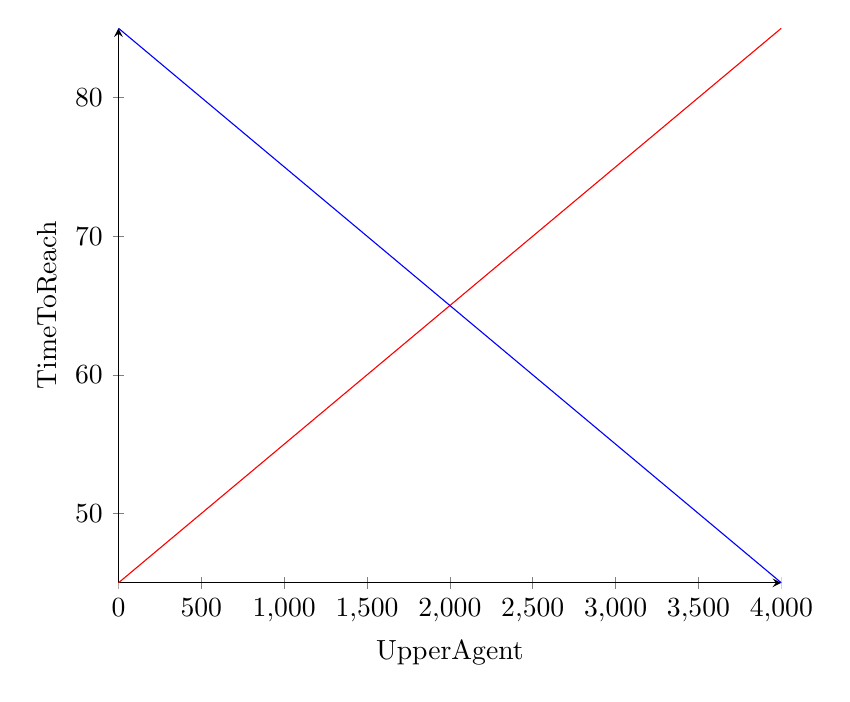
\begin{tikzpicture}
\begin{axis}[
    axis lines = left,
    xlabel = UpperAgent,
    ylabel = TimeToReach,
]
%Below the red parabola is defined
\addplot [
    domain=0:4000, 
    samples=100, 
    color=red,
]
{x/100 + 45};
\addplot [
    domain=0:4000, 
    samples=100, 
    color=blue,
]
{85 - x/100};

\end{axis}
\end{tikzpicture}
\end{center}
Red is upper agents and blue is lower agents.\\
The Only Point that two Best-Response meet as on (2000, 2000).

\subexercise
\[
U_{x} = 
     \begin{cases}
      {x \over 100} + 45 &\quad\text {if x Agent choose Upper} \\
      40 + {k\over 100} &\quad\text{if k Agent from X choose C-D}\\ 
      45 + {4000 - x + k \over 100} &\quad\text{otherwise}\\ 
     \end{cases}
\]
First we find all Nash points in upper and mid road and then check if the answer can be used applied in case three road exists.
\begin{equation} \label{eq1}
\begin{split}
    U_{upper} & = U_{mid}\\
    {x \over 100} + 45 & = 40 + {k \over 100}\\
    x & = k - 500
\end{split}
\end{equation}
\[
U_{x} = 
     \begin{cases}
      {x \over 100} + 45 &\quad\text {if x Agent choose Upper} \\
      45 + {x\over 100} &\quad\text{if k Agent from X choose C-D}\\ 
      85 &\quad\text{otherwise}\\ 
     \end{cases}
\]

\begin{center}
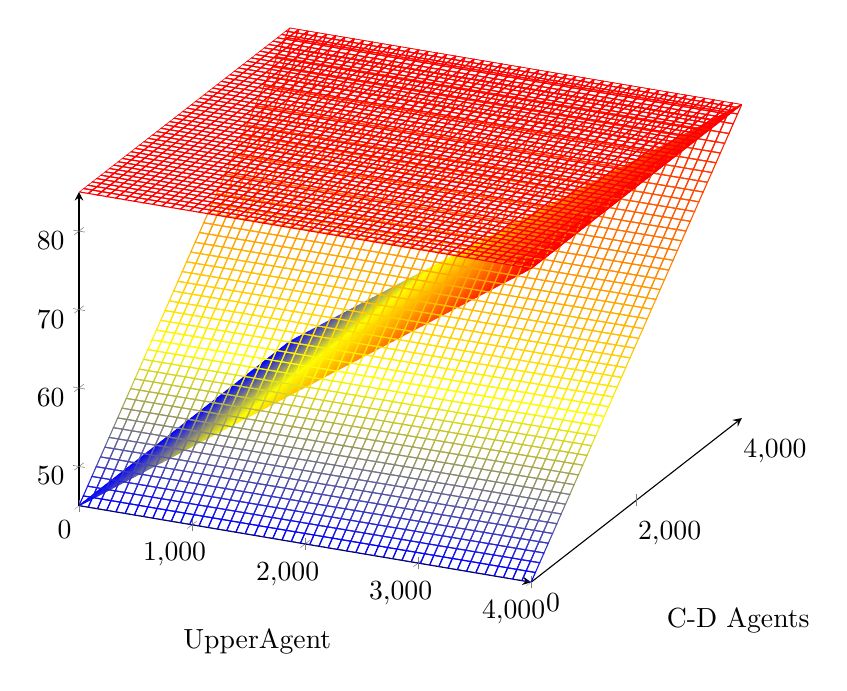
\begin{tikzpicture}
\begin{axis}[
    axis lines = left,
    xlabel = UpperAgent,
    ylabel = C-D Agents,
]
%Below the red parabola is defined
\addplot3[
    mesh,
    samples=50,
    domain=0:4000,
    % color=blue,
]
{x/100 + 45};
\addplot3[
    mesh,
    samples=50,
    domain=0:4000,
    % color=red,
]
{45 + y/100};
\addplot3[
    mesh,
    samples=50,
    domain=0:4000,
    % color=green,
]
{85};
\end{axis}
\end{tikzpicture}
\end{center}
The Only Point that all surface meet as on (4000, 4000, 85).\\
It means Nash happen when all agents take A-C-D-B road and cost is 85.\\
Surprisingly adding a new road with cost 0 moved Nash from 65 to 85.

\subexercise
Some basic mathematical notation: normally, one needs to write \texttt{\textbackslash{}mathbb\{R\}} to get~$\R$, but we have defined shortcuts for you: \texttt{\textbackslash{}R} works!
\[ \R \quad \N \quad \Z \quad \Q \quad < \quad > \quad \leq \quad \geq \quad \neq \quad x^2 \quad \sqrt{y} \]
\[ 3 \cdot 3 = 3^2 = 9 \]

\subexercise
Here's a math table-like environment for setting up a series of derivations.
\begin{eqnarray*}
  && T \\
  &\equiv& \{ \text{rule to be proven } \Rightarrow \} \\
  && ? \\
  &\equiv& \{ \text{rule to be proven } \wedge \} \\
  && F
\end{eqnarray*}

But if you don't want to use (a lot of) math inside a table, a normal table also works:
\begin{center}
  \begin{tabular}{lcr}
    \toprule
    left & center & right \\
    \midrule
    l & c & r \\
    $x+y$ & $\equiv$ & $y + x$ \\
    \bottomrule
  \end{tabular}
  %
  \hspace{5em}
  %
  \begin{tabular}{rl}
    & $a \vee b$ \\
    & $\neg a$ \\
    \hline
    $\therefore$ & $b$
  \end{tabular}
\end{center}


\exercise

\subexercise Regular expressions can be written as: $(a + \varepsilon)^* (a+b) ab$.
\subexercise Useful for writing about Turing machines, but also for concluding a proof: $\square$.

In fact, we can write a proof as follows.

\begin{proof}
  It can easily be seen that this statement is concluded with a \texttt{\textbackslash{}qed} symbol.
\end{proof}


\exercise

We can specify an algorithm in pseudo-code as follows.

\begin{algorithm}[H]
  \caption{MyIncredibleAlgorithm($A, v$)}
  \KwIn{an array $A$ of $n$ numbers and a number $v$}
  \KwOut{an index $i$ such that $A[i] = 42$, or \textsc{NotFound} if no such index exists}

  $i \leftarrow 1$ \;
  \While{$i \leq n$ \And $A[i] \neq 42$}{
    $A[i].\textit{update()}$ \;
    $i \leftarrow i + v^2$
  }
  \tcc{the following loop runs over all of $A$}
  \For(\tcp*[f]{use a different indicator variable here}){$j \leftarrow 1$ \To $n$}{
    something useful \tcp*{you can write text if that's more succinct}
    \If{$j$ is even}{
      $A[j].\textit{flip()}$
    }
  }
  \leIf{$i > n$}{
    \Return{\textsc{NotFound}}
  }{
    \Return{$i$}
  }
\end{algorithm}

\noindent For analysis, you may want to know $O, \Theta, \Omega(n \log n)$ (not to be confused with $o, \omega$).


\exercise

A figure (such as Figure~\ref{fig:squares}) can be inserted, PDF format is preferred.

\begin{figure}[b] % The letters between square brackets tell LaTeX where the figure can be placed:
  % `h` means 'right here';
  % `b` means 'at the bottom of the page';
  % `t` means 'at the top of the page';
  % `p` means 'at a separate page (optionally with other figures if that fits).
  % Specifying only `h` will not work, LaTeX will automatically change that to `ht`.
  \begin{center}
    \includegraphics{squares}
    \caption{Three axis-aligned squares.}
    \label{fig:squares}
  \end{center}
\end{figure}

To insert a figure precisely where you want it to appear, you can leave away the \texttt{figure} environment. You will then however not be able to add a caption or refer to it.

\begin{center}
  \includegraphics{squares}
\end{center}

The caption of Figure~\ref{fig:squares} can be left away completely, but you will not be able to refer to the figure anymore if you do that; the \texttt{\textbackslash{}label} only works right after a \texttt{\textbackslash{}caption}. Note how \LaTeX{} can automatically fill in the figure number for you, making it easy to refer to figures. The same approach works for tables, although it is common practice to put the caption before the table instead of below it; this can be seen in Table~\ref{tab:courses}.

\begin{table}[bt]
  \caption{Courses taught by members of the Applied Geometric Algorithms group.}
  \label{tab:courses}
  \begin{center}
    \begin{tabular}{ll}
      \toprule
      \textbf{Course code} & \textbf{Course name} \\
      \midrule
      2IL50 & Data Structures \\
      JBI020 & Foundations of Computing \\
      \bottomrule
    \end{tabular}
  \end{center}
\end{table}

\subexercise
As you can see, you can put text before the first subexercise as well, if you wish.

\exercise[6]
\subexercise[b]
You can explicitly state the exercise too. This is useful if you cannot answer all questions.

\subexercise
Further subexercises can be numbered automatically again.

\exercise
The numbering will continue where it left off.

\end{document}
